\section{Iteración 1}
\label{sec:iteracion_1}

% Para la primera iteración se implementaron las historias de usuario con más relevancia dentro de la lógica de negocio del cliente, estas son generalmente las que tienen mayor impacto en el sistema a desarrollar. \\

%
% \subsection{Iteration Planning Meeting}
% \label{sub:Iteration Planning Meeting}

\subsection{Planificación}

En esta etapa se analizaran las Historias de Usuario seleccionadas para esta iteración, y se las dividirá en \emph{tareas de ingeniería}. \\

% \begin{itemize}
%   \item \textbf{Planificación de la Iteración 1:} En esta etapa se analizan las Historias de Usuario seleccionadas para esta iteración, y se las divide en \emph{tareas de ingeniería}.
% \end{itemize}
  %
  % \subsection{Exploración y Planeación}
  % \label{subs:Exploración y Planeación}


% En un equipo de desarrollo formado por varias personas, las fases de Exploración y Planeación se las realiza por separado, primeramente en la fase de \emph{exploración} los desarrolladores se apropian de alguna de las historias de usuario planeadas para la iteración y procede a dividir la historia de usuario en \emph{Tareas de Ingeniería}, posteriormente en la fase de la \emph{Planeación}, todos los desarrolladores estiman las tareas de acuerdo a criterio propio. \\
%
% Tomando en cuenta que el equipo de desarrollo está compuesto solo por mi persona, para la implementación del presente proyecto de grado, las fases de Exploración y Planeación se las realizó al mismo tiempo. \\
%
% Para la primera iteración se determinó que las historias de usuario a implementar serían la 1 y la 2.   \\
% %
% Posteriormente como tarea del desarrollador se procede a dividir las historias de usuario en Tareas de Ingeniería, en la tabla se determinaron las Tareas pertenecientes a la historia de usuario 2, dentro lo que es la planeación se debe repartir las tareas entre los desarrolladores, pero ya que el equipo de desarrollo se traduce a mi persona, todas las tareas recaen sobre mi responsabilidad, como parte de la planeación es necesario estimar las tareas,

% En esta etapa se analizan las Historias de Usuario seleccionadas para esta iteración, y se las divide en \emph{tareas de ingeniería}.

  % \subsubsection{Tareas del US01}
  % \label{sub:us01_tasks}

En primer lugar se analizará la \emph{historia de usuario} US01, tal como se puede ver en el cuadro \ref{tab:US01}.

  
\begin{table}[H]
  \begin{center}
    \begin{tabularx}{0.75\textwidth}{ X }
      \toprule
      \textbf{Historia de Usuario:} US01
      \makebox[6cm][r]{\textbf{Prioridad:} Alta \space} \\
      \makebox[4cm][r]{}
      \makebox[6cm][r]{\textbf{Riesgo:} Medio} \\
      \textbf{Nombre:} Implementar la lista de lugares.\\

      % \textbf{Prioridad:} Alta \\
      % \textbf{Riesgo:} Alta \\

      % \addlinespace
      % \textbf{Nombre:} Verificar el Formulario de Registro \\

      \addlinespace
      \textbf{Descripción:} \\
      \tab Yo como visitante\\
      \tab Deseo ver una lista de lugares \\
      % & Deseo ingresar el nombre de un lugar\\
      \tab Para encontrar el lugar al que deseo ir\\

      \addlinespace
      \textbf{Criterios de Aceptación:} \\
      \tab Quiero tener los lugares en una base de datos \\
      \tab Quiero ver una lista de lugares\\
      \tab Quiero filtrar la lista de lugares por el nombre o parte de este\\

      \bottomrule
    \end{tabularx}
    \caption{Historia de Usuario - US01}
    \label{tab:US01}
  \end{center}
\end{table}


    \begin{table}[H]
  \begin{center}
    \begin{tabularx}{0.75\textwidth}{ X }
      \toprule
      \textbf{Número de Tarea:} T001
      \makebox[1cm][r]{}
      \makebox[6cm][r]{\textbf{Historia de Usuario:} US01} \\

      \addlinespace
      \textbf{Descripción:} Crear un archivo shapefile con información inicial de lugares principales dentro el campus de la UMSS. \\

      \addlinespace
      \textbf{Tipo de Tarea:} Desarrollo
      % \makebox[1cm][r]{}
      \makebox[6cm][r]{\textbf{Estimación [dias]:} 1} \\

      \addlinespace
      \textbf{Programador Responsable:} Edmundo Figueroa \\

      \bottomrule
    \end{tabularx}
    \caption{Tarea de Ingeniería - T001}
    \label{tab:T001}
  \end{center}
\end{table}


\begin{table}[H]
  \begin{center}
    \begin{tabularx}{0.75\textwidth}{ X }
      \toprule
      \textbf{Número de Tarea:} T002
      \makebox[1cm][r]{}
      \makebox[6cm][r]{\textbf{Historia de Usuario:} US01} \\

      \addlinespace
      \textbf{Descripción:} Crear una base de datos que pueda manejar información geoespacial. \\

      \addlinespace
      \textbf{Tipo de Tarea:} Desarrollo
      % \makebox[1cm][r]{}
      \makebox[6cm][r]{\textbf{Estimación [dias]:} 1} \\

      \addlinespace
      \textbf{Programador Responsable:} Edmundo Figueroa \\

      \bottomrule
    \end{tabularx}
    \caption{Tarea de Ingeniería - T002}
    \label{tab:T002}
  \end{center}
\end{table}

\begin{table}[H]
  \begin{center}
    \begin{tabularx}{0.75\textwidth}{ X }
      \toprule
      \textbf{Número de Tarea:} T003
      \makebox[1cm][r]{}
      \makebox[6cm][r]{\textbf{Historia de Usuario:} US01} \\

      \addlinespace
      \textbf{Descripción:} Popular la base de datos creada en T002 con la información de T001. \\

      \addlinespace
      \textbf{Tipo de Tarea:} Desarrollo
      \makebox[6cm][r]{\textbf{Estimación [dias]:} 0.5} \\

      \addlinespace
      \textbf{Programador Responsable:} Edmundo Figueroa \\

      \bottomrule
    \end{tabularx}
    \caption{Tarea de Ingeniería - T003}
    \label{tab:T003}
  \end{center}
\end{table}

\begin{table}[H]
  \begin{center}
    \begin{tabularx}{0.75\textwidth}{ X }
      \toprule
      \textbf{Número de Tarea:} T004
      \makebox[1cm][r]{}
      \makebox[6cm][r]{\textbf{Historia de Usuario:} US01} \\

      \addlinespace
      \textbf{Descripción:} Mostrar una lista de los lugares. \\

      \addlinespace
      \textbf{Tipo de Tarea:} Desarrollo
      \makebox[6cm][r]{\textbf{Estimación [dias]:} 2} \\

      \addlinespace
      \textbf{Programador Responsable:} Edmundo Figueroa \\

      \bottomrule
    \end{tabularx}
    \caption{Tarea de Ingeniería - T004}
    \label{tab:T004}
  \end{center}
\end{table}


\begin{table}[H]
  \begin{center}
    \begin{tabularx}{0.75\textwidth}{ X }
      \toprule
      \textbf{Número de Tarea:} T005
      \makebox[1cm][r]{}
      \makebox[6cm][r]{\textbf{Historia de Usuario:} US01} \\

      \addlinespace
      \textbf{Descripción:} Filtrar los lugares ingresando el nombre o parte de este. \\

      \addlinespace
      \textbf{Tipo de Tarea:} Desarrollo
      \makebox[6cm][r]{\textbf{Estimación [dias]:} 1} \\

      \addlinespace
      \textbf{Programador Responsable:} Edmundo Figueroa \\

      \bottomrule
    \end{tabularx}
    \caption{Tarea de Ingeniería - T005}
    \label{tab:T005}
  \end{center}
\end{table}


  % \subsubsection{Tareas del US02}
  % \label{sub:us02_tasks}

Posteriormente se analizará la la \emph{historia de usuario} US02, ver el cuadro \ref{tab:US02}.

  
\begin{table}[H]
 \begin{center}
   \begin{tabularx}{0.75\textwidth}{ X }
     \toprule
     \textbf{Historia de Usuario:} US02
     \makebox[6cm][r]{\textbf{Prioridad:} Baja} \\
     \makebox[4cm][r]{}
     \makebox[6cm][r]{\textbf{Riesgo:} Alto} \\

     \addlinespace
     \textbf{Nombre:} Implementar la vista de la información del lugar.\\
     
     \addlinespace
     \textbf{Descripción:} \\
     \tab Yo como visitante\\
     \tab Deseo ver la información de un lugar\\
     % & Deseo ingresar el nombre de un lugar\\
     \tab Para decidir si es el lugar que estoy buscando\\

     \addlinespace
     \textbf{Criterios de Aceptación:} \\
     \tab Quiero leer una descripción del lugar \\
     \tab Quiero ver un teléfono asociado al lugar\\
     \tab Quiero ver en qué piso se encuentra el lugar\\

     \bottomrule
   \end{tabularx}
   \caption{Historia de Usuario - US02}
   \label{tab:US02}
 \end{center}
\end{table}


    \begin{table}[H]
  \begin{center}
    \begin{tabularx}{0.75\textwidth}{ X }
      \toprule
      \textbf{Número de Tarea:} T006
      \makebox[1cm][r]{}
      \makebox[6cm][r]{\textbf{Historia de Usuario:} US02} \\

      \addlinespace
      \textbf{Descripción:} Mostrar la Descripcion del lugar. \\

      \addlinespace
      \textbf{Tipo de Tarea:} Desarrollo
      \makebox[6cm][r]{\textbf{Estimación [dias]:} 0.5} \\

      \addlinespace
      \textbf{Programador Responsable:} Edmundo Figueroa \\

      \bottomrule
    \end{tabularx}
    \caption{Tarea de Ingeniería - T006}
    \label{tab:T006}
  \end{center}
\end{table}


\begin{table}[H]
  \begin{center}
    \begin{tabularx}{0.75\textwidth}{ X }
      \toprule
      \textbf{Número de Tarea:} T007
      \makebox[1cm][r]{}
      \makebox[6cm][r]{\textbf{Historia de Usuario:} US02} \\

      \addlinespace
      \textbf{Descripción:} Mostrar el telefono del lugar. \\

      \addlinespace
      \textbf{Tipo de Tarea:} Desarrollo
      % \makebox[1cm][r]{}
      \makebox[6cm][r]{\textbf{Estimación [dias]:} 0.5} \\

      \addlinespace
      \textbf{Programador Responsable:} Edmundo Figueroa \\

      \bottomrule
    \end{tabularx}
    \caption{Tarea de Ingeniería - T007}
    \label{tab:T007}
  \end{center}
\end{table}

\begin{table}[H]
  \begin{center}
    \begin{tabularx}{0.75\textwidth}{ X }
      \toprule
      \textbf{Número de Tarea:} T008
      \makebox[1cm][r]{}
      \makebox[6cm][r]{\textbf{Historia de Usuario:} US02} \\

      \addlinespace
      \textbf{Descripción:} Mostrar el nivel o el piso del lugar. \\

      \addlinespace
      \textbf{Tipo de Tarea:} Desarrollo
      \makebox[6cm][r]{\textbf{Estimación [dias]:} 0.5} \\

      \addlinespace
      \textbf{Programador Responsable:} Edmundo Figueroa \\

      \bottomrule
    \end{tabularx}
    \caption{Tarea de Ingeniería - T008}
    \label{tab:T008}
  \end{center}
\end{table}

\begin{table}[H]
  \begin{center}
    \begin{tabularx}{0.75\textwidth}{ X }
      \toprule
      \textbf{Número de Tarea:} T009
      \makebox[1cm][r]{}
      \makebox[6cm][r]{\textbf{Historia de Usuario:} US02} \\

      \addlinespace
      \textbf{Descripción:} Mostrar una imagen o foto del lugar. \\

      \addlinespace
      \textbf{Tipo de Tarea:} Desarrollo
      \makebox[6cm][r]{\textbf{Estimación [dias]:} 2} \\

      \addlinespace
      \textbf{Programador Responsable:} Edmundo Figueroa \\

      \bottomrule
    \end{tabularx}
    \caption{Tarea de Ingeniería - T009}
    \label{tab:T009}
  \end{center}
\end{table}


    %
    % \begin{itemize}
    %   \item \textbf{Implementación de la Iteración 1:}
    % \end{itemize}




\subsection{Diseño}


\begin{itemize}
  \item \textbf{Diagrama Entidad - Relación:}

En la figura \ref{fig:er_lugar}, se observa el diagrama Entidad - Relación correspondiente a los \emph{lugares} dentro del campus Universitario.

\begin{figure}[H]
  \begin{center}
    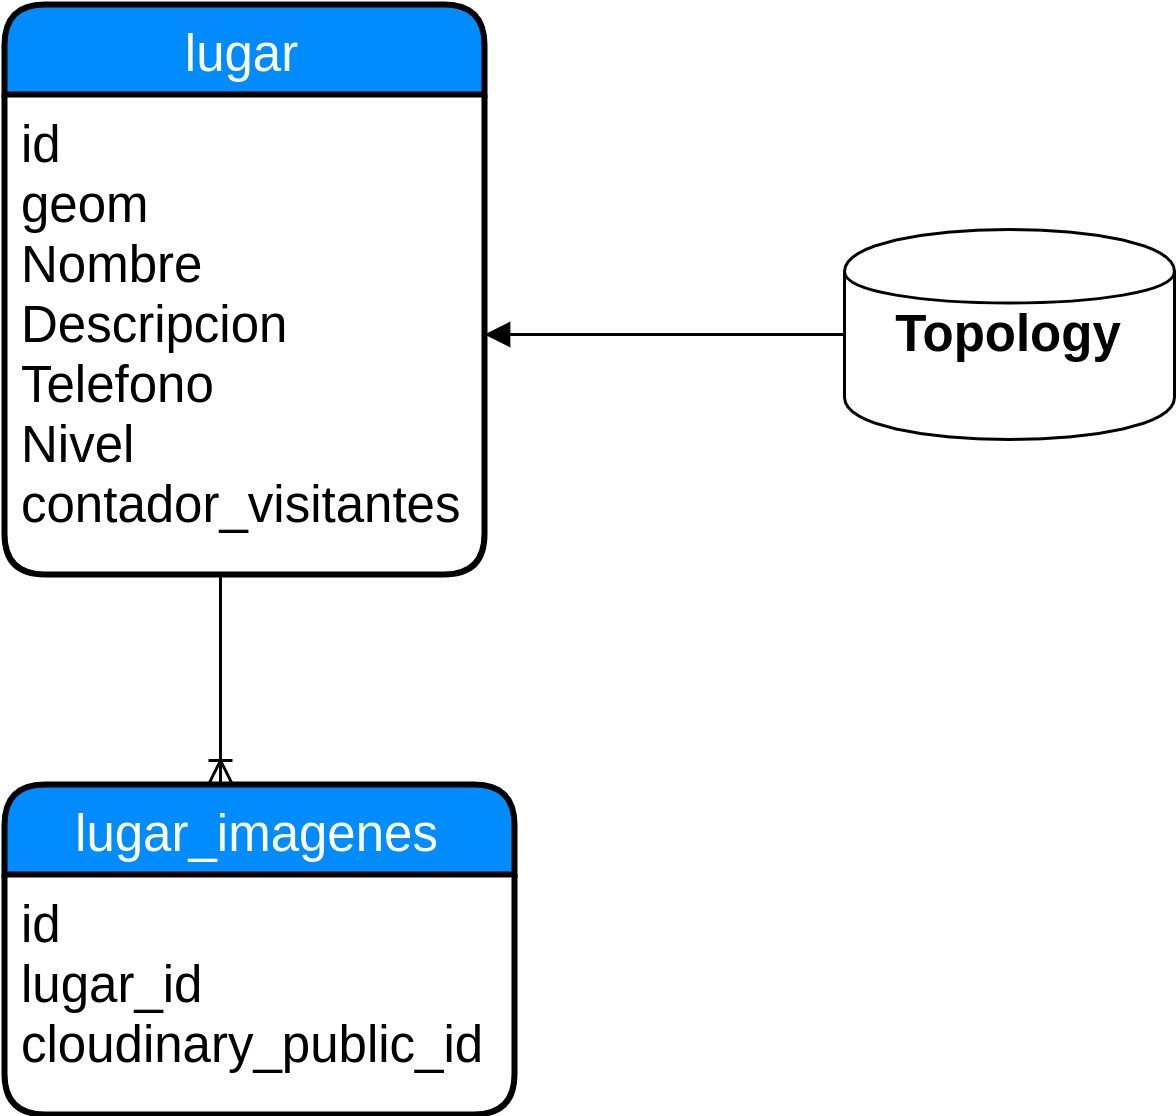
\includegraphics[width=0.4\textwidth]{diagramas/er_lugar}
  \end{center}
  \caption{Diagrama ER: Lugares}
  \label{fig:er_lugar}
  \caption*{Fuente: Elaboración propia}
\end{figure}



\item \textbf{Diagrama de Secuencia:}

En la figura \ref{fig:sequence_ver_lugar}, se observa el diagrama de secuencia correspondiente obtención de la lista e información de lugares.


\begin{figure}[H]
  \begin{center}
    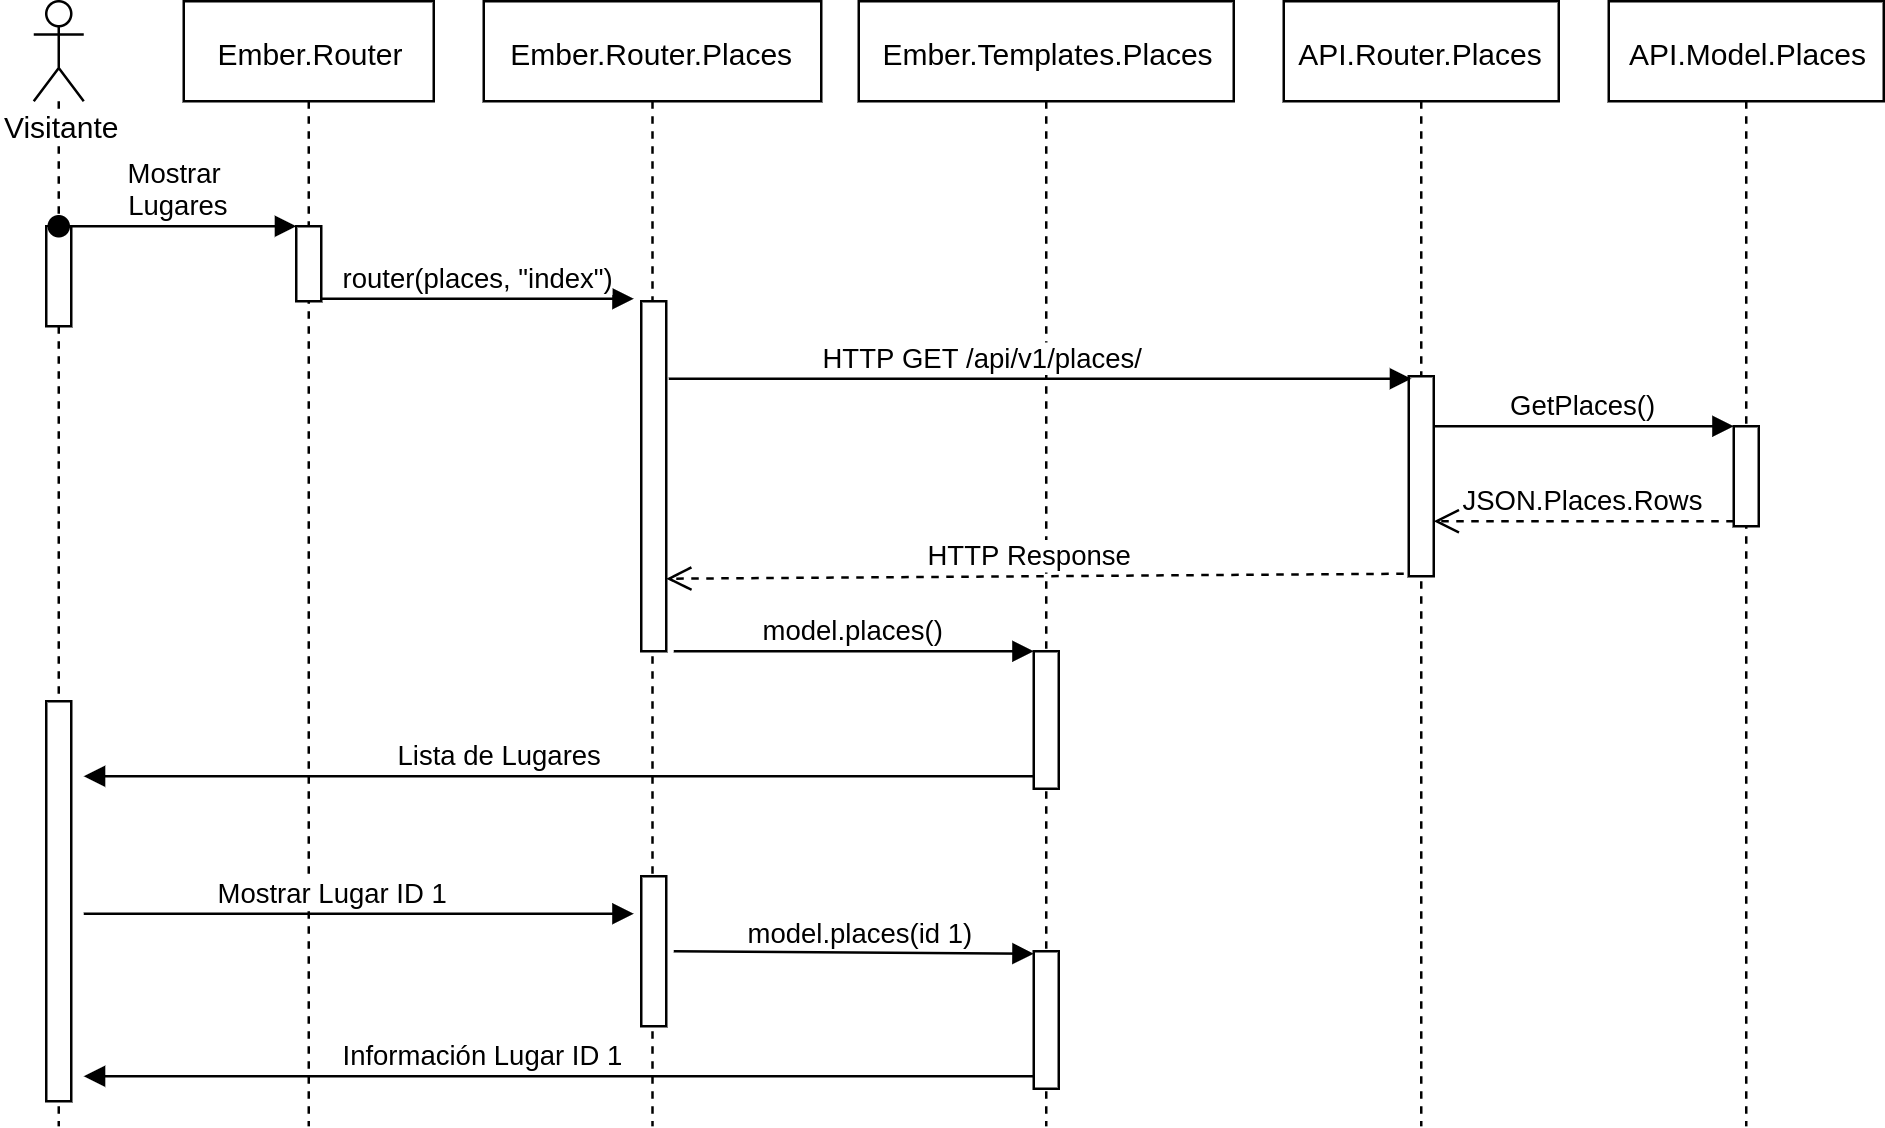
\includegraphics[width=0.9\textwidth]{diagramas/sequence_ver_lugar}
  \end{center}
  \caption{Diagrama de Secuencia: Lista e Información de Lugares}
  \label{fig:sequence_ver_lugar}
  \caption*{Fuente: Elaboración propia}
\end{figure}



\item \textbf{Diagrama de Clases:}


En la figura \ref{fig:clases_lugares}, se observa el diagrama de clases correspondiente a los lugares y la información de estos.

\begin{figure}[H]
\begin{center}
  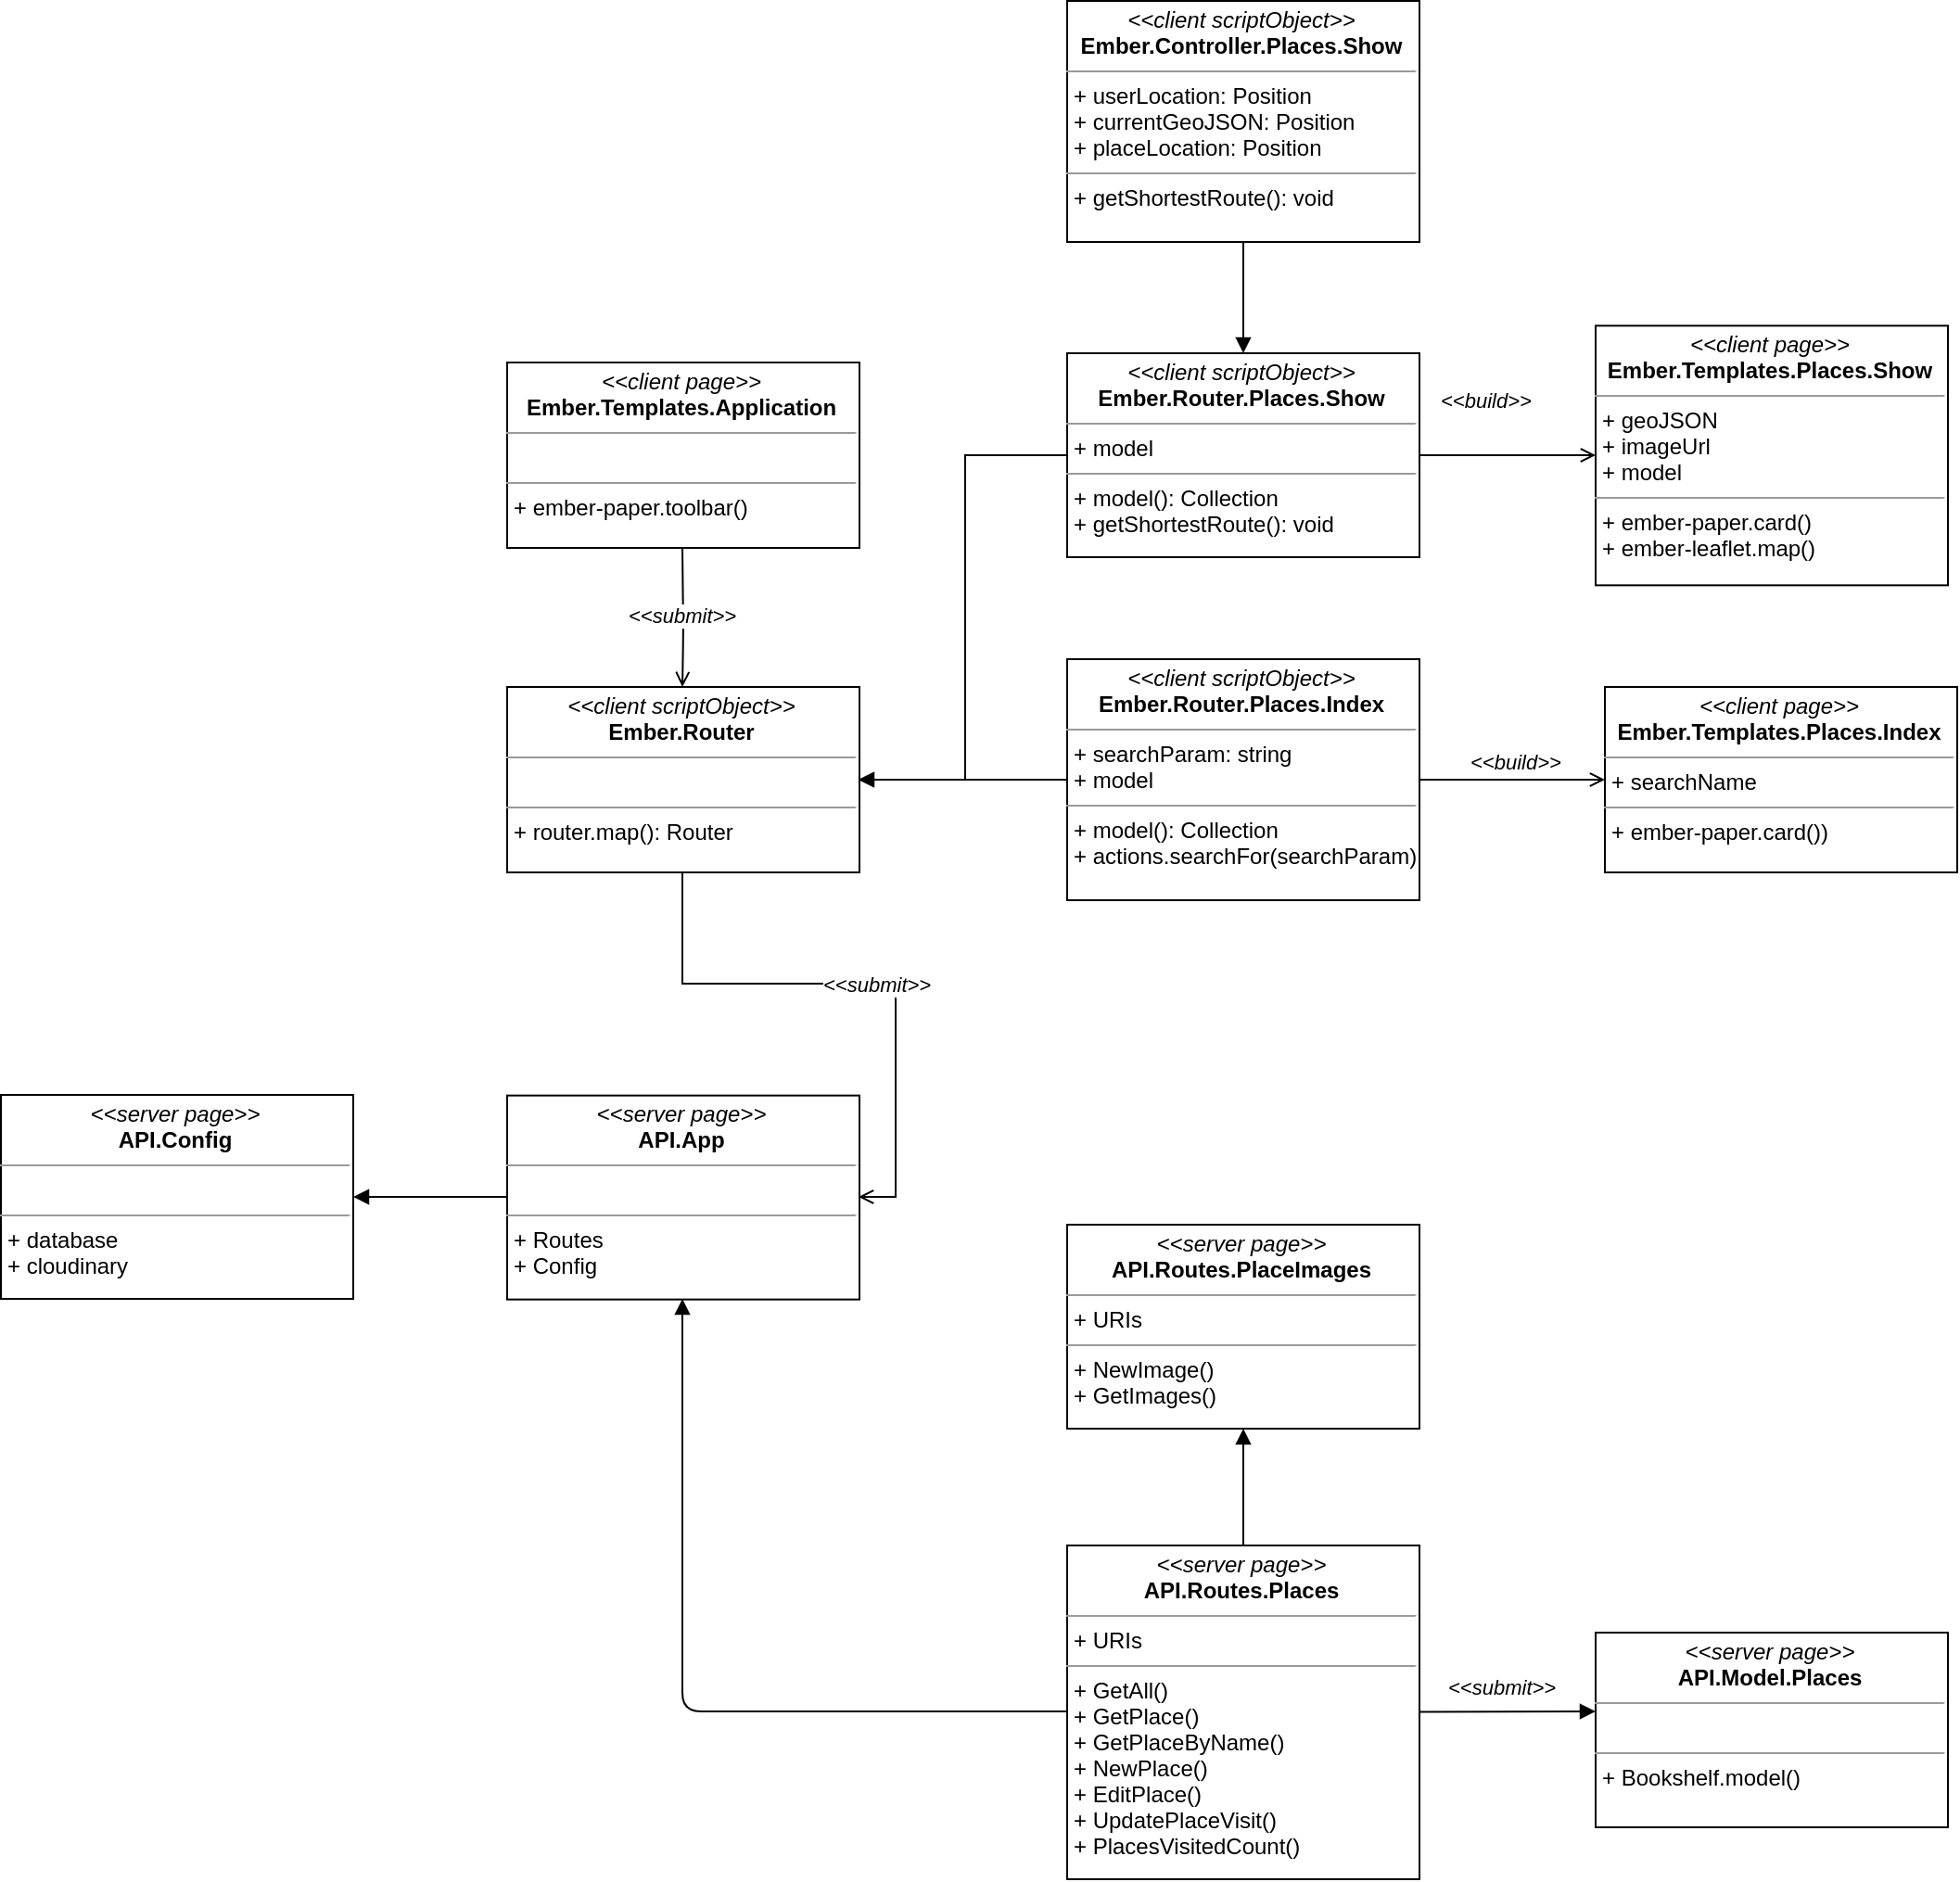
\includegraphics[width=0.9\textwidth]{diagramas/clases_lugares}
\end{center}
\caption{Diagrama de Clases: Lugares}
\label{fig:clases_lugares}
\caption*{Fuente: Elaboración propia}
\end{figure}


\end{itemize}


\subsection{Implementación}
% \label{sub:implementacion_iteracion_1}

    \subsubsection{Recolecion de la informacion de los lugares}
% \label{subs:Los lugares}

En primer lugar se recolectó la información de los lugares que la aplicación contendrá  de forma inicial, al igual que para recolectar las rutas se hizo uso de un \emph{GPS Garmin Nuvi 1300}, el cual cuenta con la opción de guardar locaciones como favoritos, entonces solo fue necesario estar cerca del lugar que se desea guardar y activar esa opción del GPS, este guarda la información en un archivo \emph{.gpx} y con la ayuda de \emph{QGIS} se genero el archivo shapefile correspondiente.\\

Posteriormente es necesario pasar la información geoespacial del shapefile a la base de datos, para esta tarea se hizo uso de una herramienta disponible para postgres, \emph{shp2pgsql}, que permite la conversión de un archivo shapefile a un archivo sql.

% $ shp2pgsql -s 4326 -I -S -c -d ~/Documents/places.shp > places.sql
\begin{verbatim}
  $ shp2pgsql -s 3785 -I -S -c -d ~/Documents/places.shp > places.sql
\end{verbatim}

Con el anterior comando se tiene como resultado un archivo \emph{.sql}, el cual es ingresado en la base de datos ya configurada, de esta forma nuestra base de datos para a contener una tabla geoespacial con datos de tipo \emph{POINT}, los cuales representan los lugares dentro del campus de la UMSS.\\

% \begin{verbatim}
%   $ shp2pgsql -s 4326 -I -S -c -d ~/Documents/ways.shp > ways.sql
% \end{verbatim}
%
% De la misma forma es necesario pasar la información de las rutas contenidas en un archivo shapefile a un archivo sql, en este caso creará una tabla \emph{WAYS}.\\

El archivo \emph{sql} resultante es usado para popular la base de datos con la información inicial de los lugares que contiene el campus universitario, para tal tarea se usó el siguiente comando.\\
% Los archivos resultantes \emph{sql} son usados para popular la base de datos .\\

\begin{verbatim}
  $ psql -d db_ubikate -U db_admin -f /Documents/places.sql
\end{verbatim}

\begin{figure}[H]
  \begin{center}
    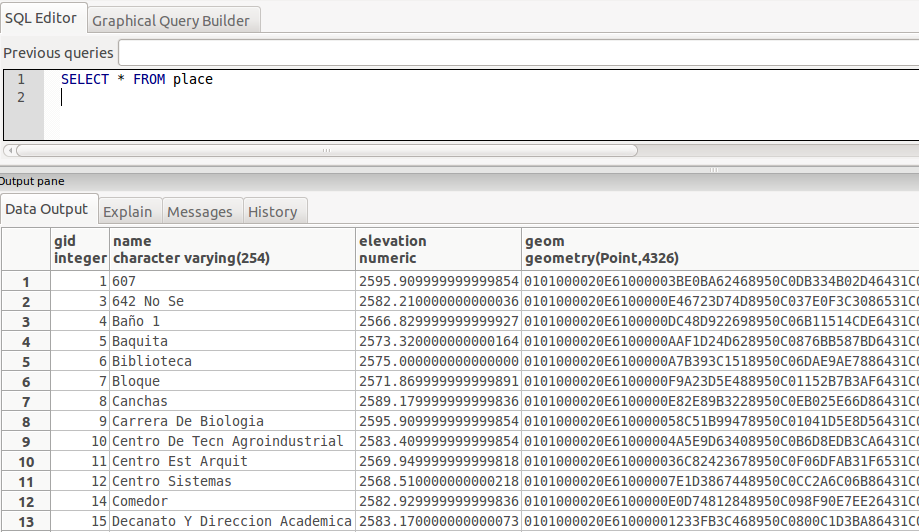
\includegraphics[width=1\textwidth]{iteration1/postgres_places}
    \caption{Herramienta gráfica de PostgreSQL (\emph{pgAdmin}).}
    \label{fig:postgres_places}
    \caption*{Fuente: Elaboración propia}
  \end{center}
\end{figure}
 % con la tabla de Lugares desplegada.

En la figura \ref{fig:postgres_places} se puede observar que la columna \emph{Elevation} contiene datos que el GPS Garmin Nuvi 1300 genera al momento de guardar un punto, en el presente caso es irrelevante.\\


Una vez que se tiene populada la base de datos con la informacion de los lugares es necesario implementar el como se comunicara el backend con el frontend, este como ya se explico se implementara un Servicio Web basado en un API REST.\\



\subsubsection{Implementación del REST API}
\label{subs:Implementacion del REST API}



El servidor necesita reconocer las peticiones que le llegan del cliente, para lo cual es necesario ``mapear'' un URI a una acción específica, las cuales ya están preparadas para comunicarse con la base de datos, no hay restricción en la declaración de las URIs pero para una mejor comprensión del API que se está desarrollando es necesario seguir convenciones que aseguran que cualquier desarrollador pueda comprender el API presentado y pueda ser fácilmente consumido por cualquier aplicación que requiera acceder a la información que disponible, un API REST es el que cumple con estas características.
En primer lugar es necesario crear las URIs que serán ``entendidas'' por el servidor, esto se logra declarando en el servicio creado con \emph{Express.JS}, tal como se puede apreciar en el siguiente bloque de código, cada URI se lo relaciona a un modelo en específico de acuerdo a la acción que se requiere, tal como se puede observar en el cuadro \ref{tab:rest} las URIs declaradas en el API cumplen con tal característica.\\


% \begin{minted}{js}[label=express_api,caption=Declarando API REST con ExpressJS]
\begin{center}
  \begin{lstlisting}[label=express_api,caption=Declarando API REST con ExpressJS]

        const router = express.Router();
        router.get('/', places.getAll);
        router.get('/:id', places.getPlace);
        router.post('/', places.newPlace);
        router.put('/:id', places.editPlace);
        router.delete('/:id', places.deletePlace);

        app.use('/api/v1/places', router);

  \end{lstlisting}
\end{center}
% \end{minted}

% En el código

  %
  % Para lograr todo este comportamiento  es necesario declarar, en el archivo
  % que controla las rutas dentro de la aplicación, \textbf{routes}, que el
  % recurso \textbf{user} es \emph{restful}, tal como se muestra en la figura \ref{fig:rest}\\

  % \begin{figure}[!hbp]
  %   \begin{center}
  %     \caption[REST - routes.rb]{config/routes.rb}
  %     \label{fig:rest}
  %     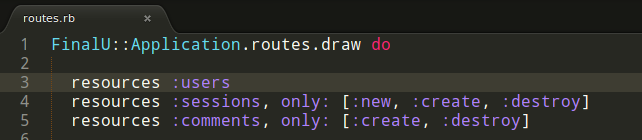
\includegraphics[width=1\textwidth]{rest}
  %     \caption*{Fuente: }
  %   \end{center}
  % \end{figure}

  El cuadro \ref{tab:rest} muestra como se puede leer las peticiones al API de \textbf{places}, las acciones mostradas son las que se pueden encontrar en un API REST pero no es necesario declararlas todas para considerar a que un API es restful.\\


  \begin{table}[H]
    \begin{center}

      \begin{tabularx}{0.75\textwidth}{ l l l  X }
        \toprule
        \multicolumn{1}{c}{\textbf{HTTP}} &
        \multicolumn{1}{c}{\textbf{URI}}  &
        % \multicolumn{1}{c}{\textbf{C}}  &
        \multicolumn{1}{c}{\textbf{ACCI\'ON}} &
        \multicolumn{1}{c}{\textbf{USADO PARA}}  \\
        \multicolumn{1}{c}{\textbf{request}} & & & \\

        \midrule
        GET     &  /places    &  index    & devuelve una lista con todos los lugares\\
        POST    &  /places    &  create   & inserta un nuevo lugar en la bd\\
        GET     &  /places/1  &  show     & muestra el lugar con identificador \emph{1}\\
        PUT     &  /places/1  &  update   & actualiza los datos de un lugar específico\\
        DELETE  &  /places/1  &  delete   & elimina el lugar con id = 1 de la bd\\
        \bottomrule
      \end{tabularx}

      \caption[recursos REST]{REST URIs para los lugares}
      \label{tab:rest}

      \caption*{Fuente: Elaboración propia}
    \end{center}
  \end{table}

  % Tal como se ve en el cuadro \ref{tab:rest}, Rails maneja los request HTTP de acuerdo con
  % el tipo de llamada que se realice, este trabajo lo realiza el \textbf{router},
  % que reconoce las URLs y los despacha a una \textbf{acción} del controlador,
  % todo este proceso ya está implementado en el núcleo de Rails por lo tanto  es automático y el programador
  % no necesita más configuración que la mostrada en la figura \ref{fig:rest},
  % obedeciendo al principio de \emph{Convención sobre configuración}\\

  % % no son más que métodos dentro del \emph{user\_controller.rb}
  % el cual
  % es parte del controlador de la arquitectura MVC.\\

  % The Rails router recognizes URLs and dispatches them to a controller’s action. It can also generate paths and URLs, avoiding the need to hardcode strings in your views.

  Por ejemplo, si se genera una petición GET hacia la direccion
  \mbox{\emph{/places/1}}  el servidor interpreta la dirección y responde
  mostrando la información del lugar “1” y en cambio si se genera
  una petición \emph{PUT} a la misma direccion \emph{/places/1} se ejecuta la acción \textbf{update} y se actualizan los datos del lugar ``1''. \\

  % \textbf{usuarios} actualizando la información del usuario “1”. \\

  Siguiendo la convención de un API REST ayuda a entender el flujo que tiene un recurso,
  las URL son legibles y únicos para cada recurso. Por lo tanto la implementación   de los recursos se hace de forma más limpia y ordenada, situaciones que son   claves para el mantenimiento y la extensibilidad del sistema. \\


Una vez implementado el servicio web, necesitamos empezar con el desarrollo del frontend de la aplicacion, que como ya se explico se usara \emph{EmberJS} para esta tarea. \\


\subsubsection{Mostrar los lugares}


\emph{EmberJS} tiene que consumir la informacion del API implementado, por lo tanto se hara una llamada \emph{GET} al URI \emph{places/}, dentro de la estructura de \emph{EmberJS} se tiene que implementar en el \emph{Router} dedicado al URI correspondiente. El siguiente metodo es el encarado de hacer la llamada y obtener la lista de lugares del API

\begin{center}
  \begin{lstlisting}[label=model_places_index,caption=Obtener la lista de lugares del API]

    model() {
        var url = (ENV.APP.API_HOST || '') + '/api/v1/places/';
        return jQuery.ajax({
          url: url,
          type: 'GET'
        });
      }

  \end{lstlisting}
\end{center}

Una vez obtenido la lista de lugares es necesario para el visitante que la lista este disponible en el navegador, para lo cual se usara el \emph{template} de \emph{EmberJs} correspondiente al URI, \emph{templates/places/index.hbs}.

\begin{center}
  \begin{lstlisting}[label=template_places_index,caption=Template de la lista de lugares]

    {{#paper-list}}
      {{#each model.data as |place|}}
        {{#paper-item class="md-1-line" onClick=(transition-to 'places.show' place)}}
            <div class="md-list-item-text">
                <span>{{place.name}}</span>
            </div>
        {{/paper-item}}
        {{paper-divider}}
      {{/each}}
    {{/paper-list}}

  \end{lstlisting}
\end{center}

En la anterior implementacion se hizo uso de \emph{ember-paper}, que como ya se explico ayudara en el ``look and feel'' de la aplicacion, el cual se puede observar en la figura \ref{fig:places_index}, la lista de lugares es mostrada en el navegador en un dispositivo movil.


\begin{figure}[H]
  \begin{center}
    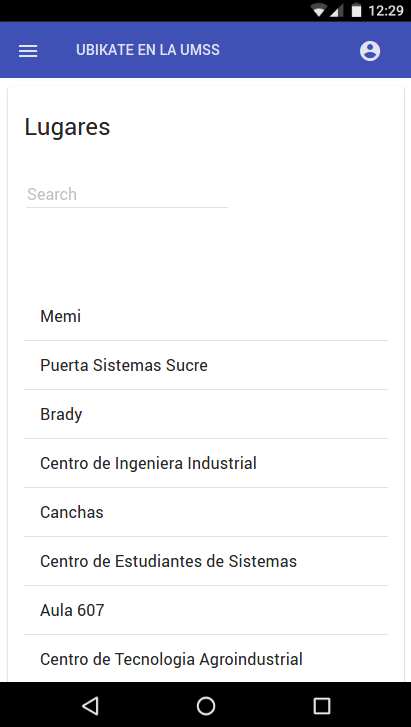
\includegraphics[width=0.3\textwidth]{iteration1/places_index_2}
    \caption{Lista de Lugares}
    \label{fig:places_index}
    \caption*{Fuente: Elaboración propia}
  \end{center}
\end{figure}


\subsubsection{Busqueda de los lugares}
\label{subs:busqueda de los lugares}

Para la implementacion de la busqueda de los lugares, un de los criterios de aceptacion es que sea posible la busqueda usando el nombre del lugar o parte del mismo, es necesario anadir un \emph{URI} adicional a nuestro servicio web, que obtenga de la base de datos un conjunto de lugares que concuerden con el criterio de busqueda, a continuacion se puede ver el URI implementado en la servicio web. \\

\begin{center}
  \begin{lstlisting}[label=endpoint_search_place,caption=Implementacion de la busqueda de lugares en el Servicio Web]

    router.get('places/search/:name', places.getPlacesByName);

  \end{lstlisting}
\end{center}


\subsubsection{Mostrar informacion del lugar}
\label{subs:Mostrar informacion del lugar}

La obtencion de la informacion de un lugar corresponde al URI \emph{places/:id} usando el verbo HTTP \emph{GET}, el cual obtiene la informacion en formato JSON, entonces se necesita mostrar esta informacion en el navegador, para lo cual el template correspondente al URI llegaria a ser \emph{templates/places/show}.

\begin{center}
  \begin{lstlisting}[label=template_places_show,caption=Template para mostrar la informacion de un lugar]
      {{#text.headline}}{{model.name}}{{/text.headline}}
      {{#card.content}}
          {{#paper-list}}
              {{model.description}}
              {{/paper-item}}
                  {{paper-icon "local_phone"}} {{model.phone}}
              {{/paper-item}}
              {{#paper-item class="md-2-line" }}
                  {{paper-icon "layers"}} Piso N# {{model.level}}
              {{/paper-item}}
          {{/paper-list}}
      {{/card.content}}

  \end{lstlisting}
\end{center}

El resultado del template renderizado en el navegador se puede apreciar en la figura \ref{fig:place_show}.

\begin{figure}[H]
  \begin{center}
    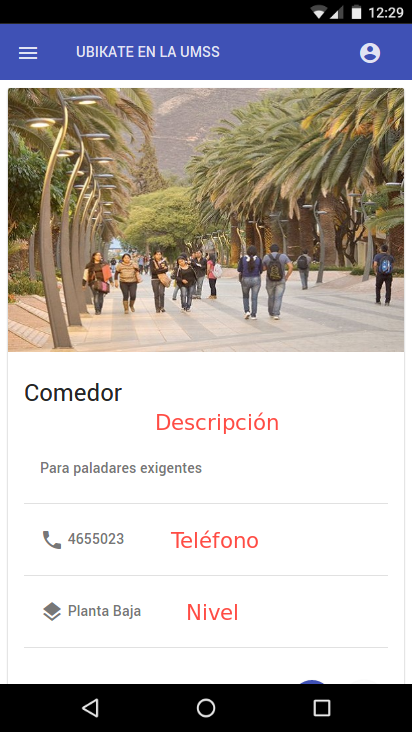
\includegraphics[width=0.3\textwidth]{iteration1/place_show}
    \caption{Vista de la Información de un Lugar.}
    \label{fig:place_show}
    \caption*{Fuente: Elaboración propia}
  \end{center}
\end{figure}




% En la figura \ref{fig:places_index}, se puede observar un


\subsection{Pruebas de Aceptación}

\begin{table}[H]
  \begin{center}
    \begin{tabularx}{0.75\textwidth}{ X }
      \toprule
      \textbf{Codigo:} CP001
      \makebox[3cm][r]{}
      \makebox[6cm][r]{\textbf{Historia de Usuario:} US01} \\

      \addlinespace
      \textbf{Nombre:} Verificar la lista de lugares. \\

      \addlinespace
      \textbf{Descripción:} Validar que un usuario visitante puede ver la lista de lugares cuando ingresa al menú \emph{lugares}. \\

      \addlinespace
      \textbf{Condiciones de Ejecución:} \\
      \tab \textbf{a.} El usuario no debe estar registrado. \\
      \tab \textbf{b.} Deben existir lugares registrados en el sistema.\\

      \addlinespace
      \textbf{Entradas / Pasos de Ejecución:}  \\
      \tab \textbf{1.} Hacer tap sobre el botón \emph{menú} en la esquina superior-izquierda. \\
      \tab \textbf{2.} Seleccionar el menú \emph{lugares}.\\

      \addlinespace
      \textbf{Resultado Esperado:} El Usuario debe ver una lista con los lugares registrados en la Condición de Ejecución \emph{b}.  \\

      \addlinespace
      \textbf{Evaluación de la Prueba:} Prueba exitosa. \\

      \bottomrule
    \end{tabularx}
    \caption{Prueba de Aceptación - CP001}
    \label{tab:CP001}
  \end{center}
\end{table}

\begin{table}[H]
  \begin{center}
    \begin{tabularx}{0.75\textwidth}{ X }
      \toprule
      \textbf{Codigo:} CP002
      \makebox[3cm][r]{}
      \makebox[6cm][r]{\textbf{Historia de Usuario:} US01} \\

      \addlinespace
      \textbf{Nombre:} Verificar la busqueda de lugares. \\

      \addlinespace
      \textbf{Descripción:} Validar que un usuario puede filtrar un lugar de la lista mediante el nombre. \\

      \addlinespace
      \textbf{Condiciones de Ejecución:} Ingresar en la base de datos el lugar con nombre ``MEMI''. \\

      \addlinespace
      \textbf{Entradas / Pasos de Ejecución:}  \\
      \tab \textbf{1.} Hacer tap sobre el botón \emph{menú} en la esquina superior-izquierda. \\
      \tab \textbf{2.} Seleccionar el menú \emph{lugares}.\\
      \tab \textbf{3.} Ingresar el nombre ``MEMI'' en el cajón de búsqueda.\\


      \addlinespace
      \textbf{Resultado Esperado:} Se debe mostrar un solo item en la lista de lugares con el nombre ``MEMI'' desplegado.\\

      \addlinespace
      \textbf{Evaluación de la Prueba:} Prueba exitosa. \\

      \bottomrule
    \end{tabularx}
    \caption{Prueba de Aceptación - CP002}
    \label{tab:CP002}
  \end{center}
\end{table}

\begin{table}[H]
  \begin{center}
    \begin{tabularx}{0.75\textwidth}{ X }
      \toprule
      \textbf{Codigo:} CP003
      \makebox[3cm][r]{}
      \makebox[6cm][r]{\textbf{Historia de Usuario:} US02} \\

      \addlinespace
      \textbf{Nombre:} Verificar la información de un lugar. \\

      \addlinespace
      \textbf{Descripción:} Validar que un usuario puede ver la descripción, el teléfono, el nivel y la foto de un lugar. \\

      \addlinespace
      \textbf{Condiciones de Ejecución:} Ingresar en la base de datos el lugar con nombre ``MEMI'' con su información completa. \\

      \addlinespace
      \textbf{Entradas / Pasos de Ejecución:}  \\
      \tab \textbf{1.} Hacer tap sobre el botón \emph{menú} en la esquina superior-izquierda. \\
      \tab \textbf{2.} Seleccionar el menú \emph{lugares}.\\
      \tab \textbf{3.} En la lista de lugares seleccionar el item ``MEMI''.\\

      \addlinespace
      \textbf{Resultado Esperado:} Se debe mostrar una pantalla con la foto del lugar ``MEMI'', su descripción, el teléfono y el nivel.\\

      \addlinespace
      \textbf{Evaluación de la Prueba:} Prueba exitosa. \\

      \bottomrule
    \end{tabularx}
    \caption{Prueba de Aceptación - CP003}
    \label{tab:CP003}
  \end{center}
\end{table}



\subsubsection{Resultado de las pruebas de la Iteración 1}

Al finalizar la Iteración 1, se ejecutaron todas las pruebas escritas durante la presente iteración, en el cuadro \ref{tab:regresion_1} se puede ver el detalle.


\begin{table}[H]
  \begin{center}
    \begin{tabularx}{0.8\textwidth}{ c  X  c }
      \toprule
        \textbf{Código} &
        \multicolumn{1}{c}{\textbf{Título de la Prueba}} &
        \textbf{Resultado}\\

      \midrule
        CP001
        &
        Verificar la lista de lugares.
        &
        Exitoso \\

\addlinespace
CP002
&
Verificar la busqueda de lugares.
&
Exitoso \\

\addlinespace
CP003
&
Verificar la información de un lugar.
&
Exitoso \\

\addlinespace
CP004
&
Verificar la lista de lugares cuando se busca un lugar no registrado.
&
Exitoso \\

\addlinespace
CP005
&
Verificar la información de un lugar mediante el URI.
&
Exitoso \\

\addlinespace
CP006
&
Verificar que el \emph{Menú} sea desplegado dinámicamente.
&
Exitoso \\



      \bottomrule
    \end{tabularx}
    \caption{Pruebas de regresión de la Iteración 1}
    \label{tab:regresion_1}
  \end{center}
\end{table}


\begin{itemize}
  \item Se ejecutaron 5 pruebas de funcionalidad, todas pasaron exitosamente.
  \item Se ejecutó 1 prueba de usabilidad, pasó exitosamente.
\end{itemize}

